\subsection{Experimental Setup}
\label{sec:experimental_setup}

\subsubsection{Scenario and Network Model}
\label{sec:scenario_setup}

All experiments were conducted on an exemplary Hamburg vertiport network. The vertiport locations are based on the Hamburg UAM scenario investigated in previous DLR studies within the HorizonUAM project~\cite{abdellaoui2025_airspace_uam,schuchardt2023_atm_uam_review}; the corridor connections between these vertiports were defined for this study to obtain a connected benchmark graph. Vertiports are represented as graph nodes corresponding to averaged pad coordinates, and air corridors are modeled as undirected edges forming a connected graph. Each corridor operates at a fixed absolute cruise layer of \SI{200}{m} above mean sea level (MSL). This fixed-altitude, obstacle-free representation is used explicitly as a benchmark abstraction for reproducible computational evaluation.

Terrain elevation and obstacle variation are therefore not modeled in this study, and the corridor layer is defined in an MSL reference to ensure comparability across experiments. Edge weights are defined by the geodesic distance between connected vertiports, computed using the Haversine formula. Accordingly, the routing cost function is purely two-dimensional and distance-based: no additional penalties or constraints for altitude variation, no-fly areas, turn costs, weather effects, or other operational factors are included in the graph search objective.

This abstraction enables reproducible shortest-path routing while preserving the geographical layout of the exemplary network. Figure~\ref{fig:hamburg_corridor_network} shows the Hamburg vertiport corridor network used for the computational evaluation.

\begin{figure}[!htbp]
    \centering
    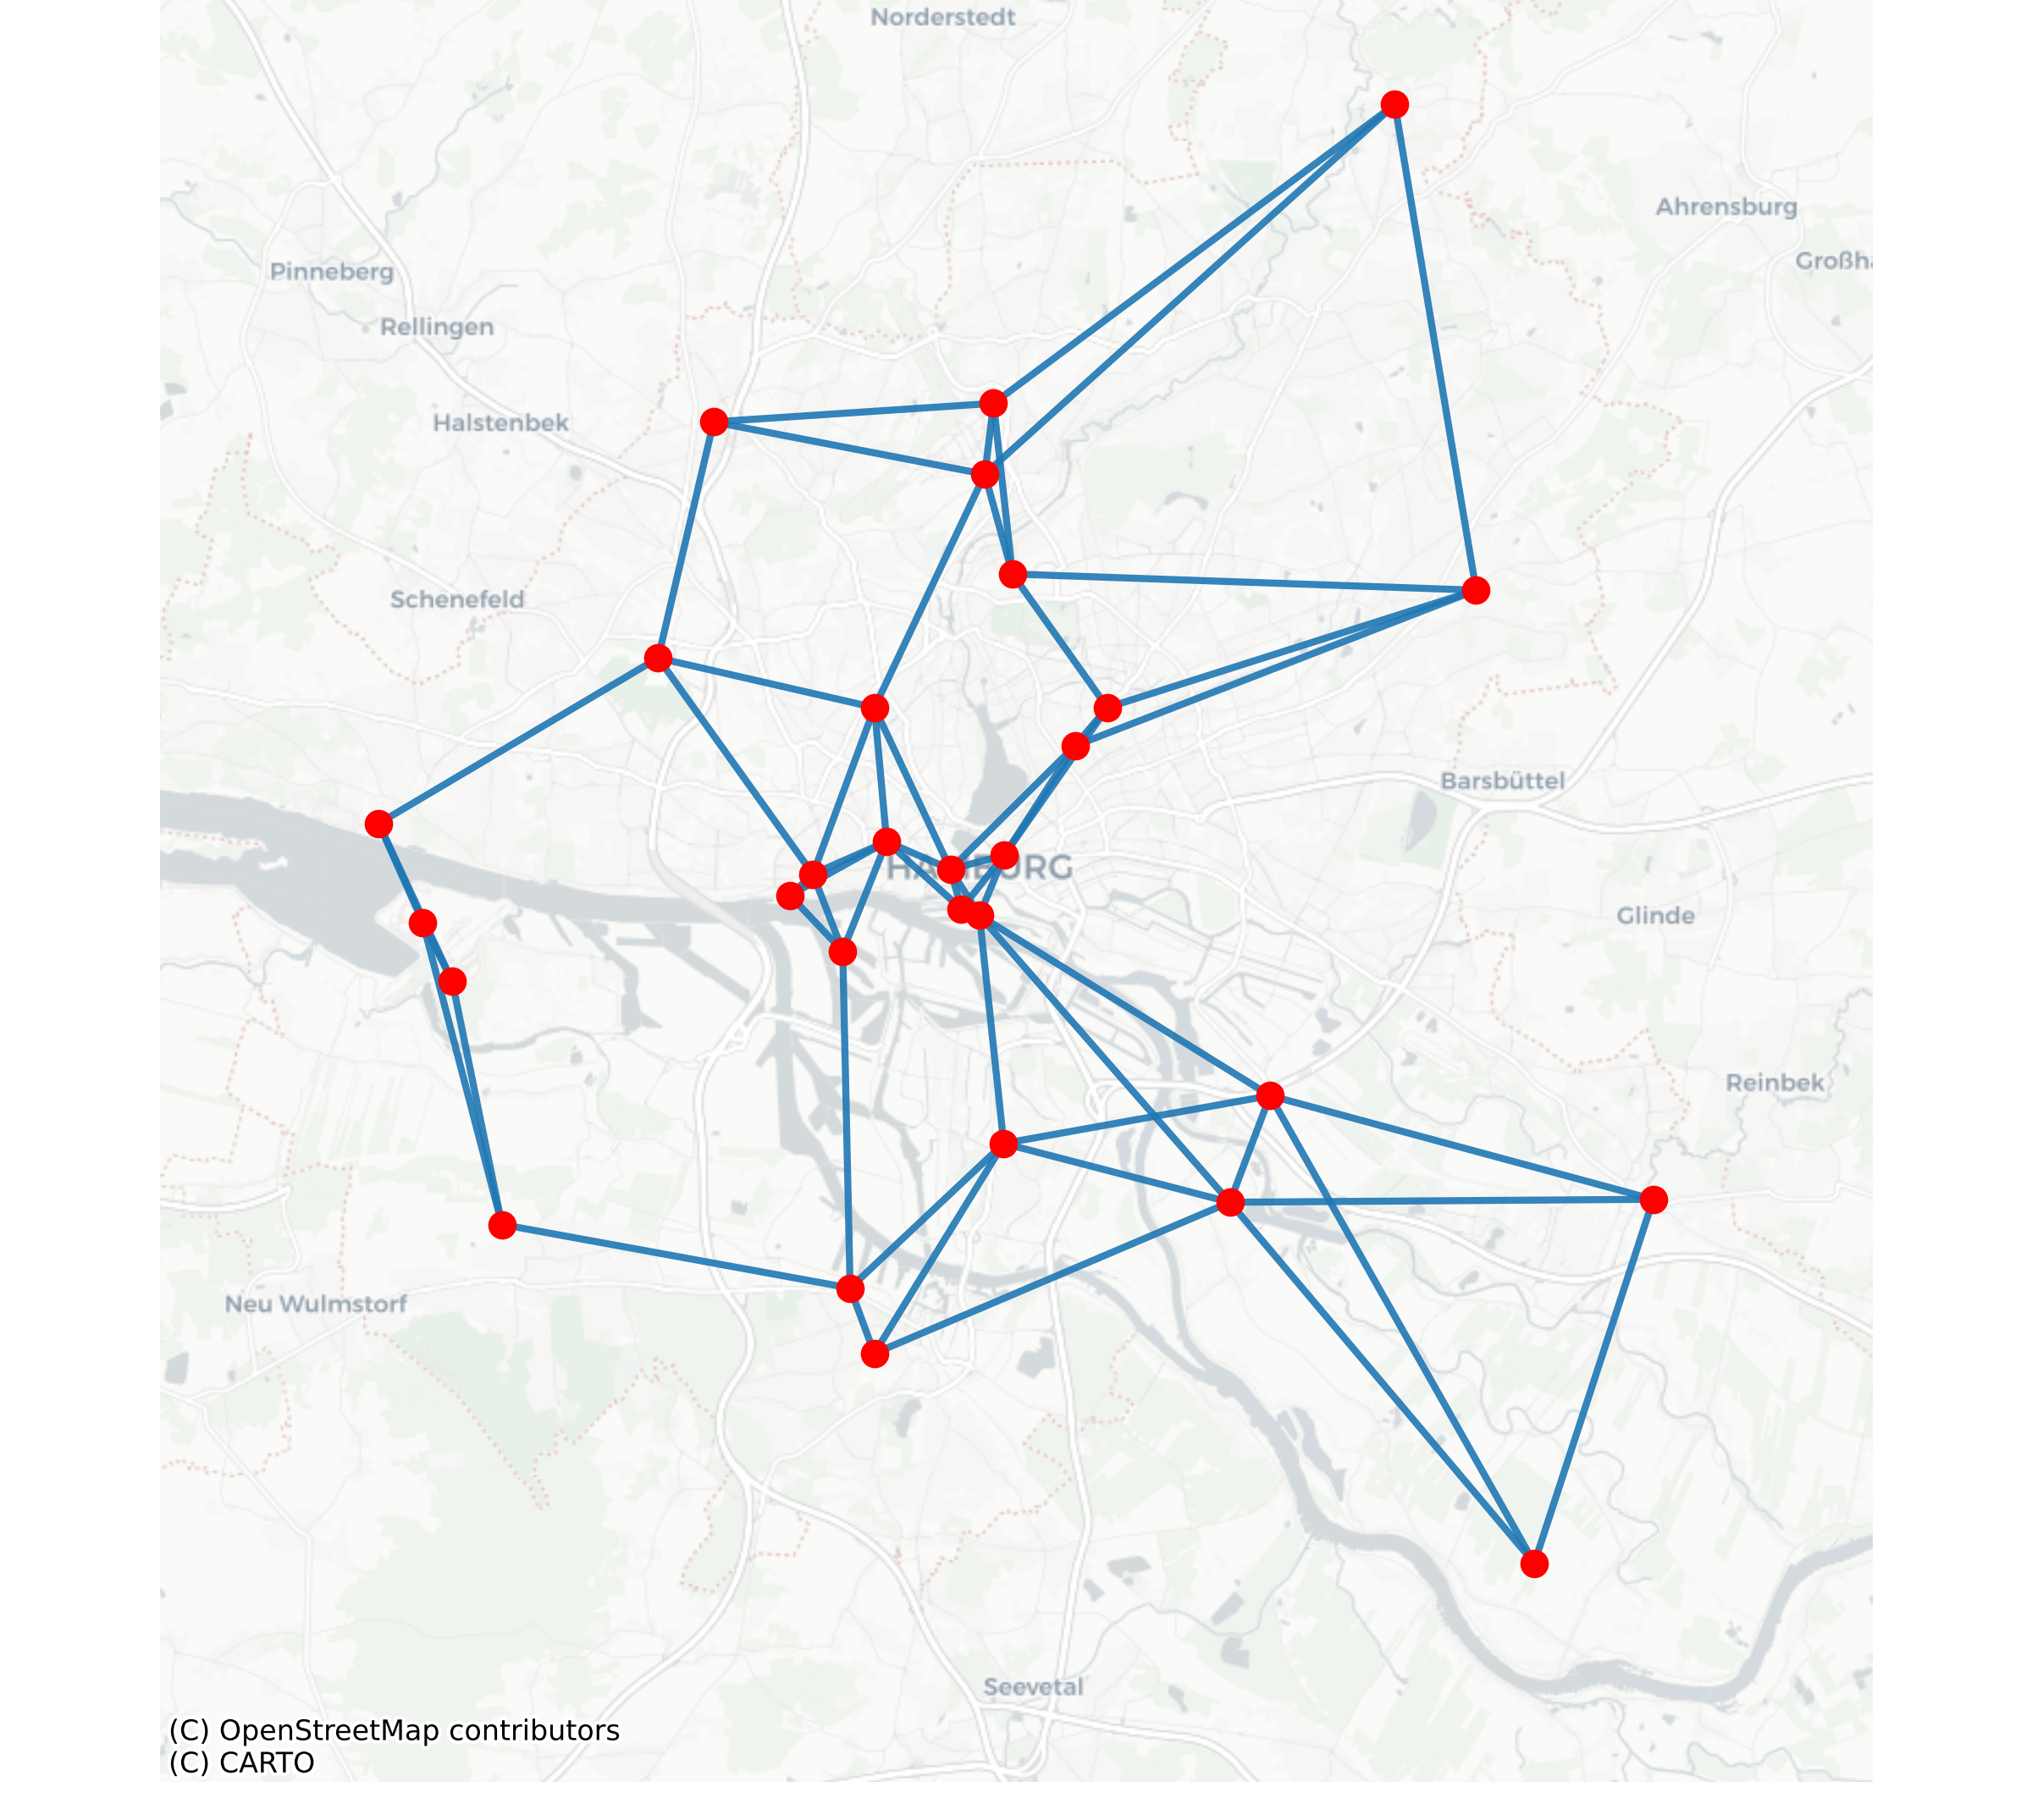
\includegraphics[
        width=0.6\linewidth
    ]{figures/hamburg_corridor_network.png}
    \caption{Hamburg vertiport corridor network used for the computational evaluation. Nodes represent vertiports and edges represent available corridor connections at the fixed \SI{200}{m} MSL cruise layer. Map data attribution: OpenStreetMap contributors and CARTO.}
    \label{fig:hamburg_corridor_network}
\end{figure}

Table~\ref{tab:network_stats} summarizes the size and basic topological properties of the analyzed vertiport network, including representative origin--destination shortest-path characteristics. The graph is small enough for fast graph search but sufficiently connected to produce multi-hop OD routes. Each undirected corridor connection is represented internally by two directed active edges, one in each travel direction.

\begin{table}[H]
    \centering
    \caption{Graph and shortest-path statistics of the analyzed vertiport network.}
    \label{tab:network_stats}
    \begin{tabularx}{\textwidth}{lX}
        \toprule
        Metric & Value \\
        \midrule
        Number of vertiports, \(|V|\) & 29 \\
        Directed active edges & 122 \\
        Undirected corridor connections & 61 \\
        Node degree range & 3--6 \\
        Mean node degree & 4.21 \\
        Median node degree & 4 \\
        Mean OD shortest-path length & 3.09 hops \\
        Median OD shortest-path length & 3 hops \\
        Mean routed OD path length & \SI{13.81}{km} \\
        Median routed OD path length & \SI{12.83}{km} \\
        \bottomrule
    \end{tabularx}
\end{table}

\subsubsection{System Configuration}
\label{sec:system_configuration}

All experiments were executed on a workstation equipped with an Intel Core i7-8650U CPU @ 1.90\,GHz with 4 cores and 8 threads, and 16\,GB RAM under a 64-bit operating system.

\begin{itemize}
    \item \textbf{Operating system:} Ubuntu 24.04 LTS (Noble Numbat).
    \item \textbf{CFMS version:} CFMS project version~1.0.
    \item \textbf{NDMap version:} Used inside the Deconfliction Service; no standalone package release is declared for the evaluated version.
\end{itemize}

The Planning Service and CFMS trajectory generator were executed locally on the same machine. The Deconfliction Service was available in the same local deployment, although the planner-stage benchmark reported below disables deconfliction to isolate routing and trajectory-generation cost. No distributed deployment, containerization, or artificial network latency was introduced. Consequently, the reported runtimes represent baseline computational performance under single-machine execution rather than distributed service latency.

The system follows a service-oriented separation of concerns; however, the evaluated deployment does not constitute a fully distributed multi-host deployment. Therefore, while the architecture supports modular decomposition, actual horizontal scaling across multiple hosts would require additional deployment mechanisms such as shared trajectory-state management, coordinated conflict-detection data access, and inter-service orchestration.

\subsubsection{Planner, Generator, and Deconfliction Configuration}
\label{sec:planner_configuration}

\begin{itemize}
    \item \textbf{Global planner:} The Planning Service performs A* search on the undirected corridor graph using Haversine distance both as edge cost and as admissible heuristic,
    \[
        f(n) = g(n) + h(n).
    \]
    The optimization objective is therefore purely 2D shortest-path distance between vertiports; altitude, no-fly constraints, and other operational cost terms are not part of the route cost model.

    \item \textbf{Deconfliction:} The Deconfliction Service invokes NDMap after CFMS-based 4D trajectory generation to evaluate the candidate trajectory against the set of already retained locally deconflicted trajectories. NDMap is not part of the Planning Service. In the implemented framework, the Deconfliction Service performs conflict detection and returns conflict information; the Planning Service performs request-local graph modification and lateral re-routing.

    \item \textbf{Cruise altitude:} A fixed absolute cruise layer of \SI{200}{m} MSL is used, independent of local pad elevation, terrain variation, and obstacle constraints. This is a benchmark assumption rather than an operational airspace model.

    \item \textbf{Waypoint synthesis:} Before CFMS execution, the planner converts each corridor route into a sparse waypoint sequence using a simplified geometry inspired by the obstacle-free-volume (OFV, ``verticone'') definitions in the EASA PTS-VPT-DSN guidance for vertical take-off and landing procedures~\cite{easa2022_pts_vpt_dsn}. For a multi-node route, the nominal sequence is:
    \begin{enumerate}
        \item origin pad waypoint,
        \item vertical climb to \(h_1\),
        \item centerline transition waypoint at \(h_2\),
        \item optional outer-limitation-surface (OLS) waypoint up to \SI{152}{m} above the pad, capped by cruise altitude,
        \item intermediate corridor nodes with altitude assigned by the design climb gradient until the fixed cruise layer is reached,
        \item optional top-of-descent waypoint on the inbound centerline,
        \item OFV entry waypoint at \(h_2\),
        \item over-pad hover waypoint at \(h_1\),
        \item landing decision point (LDP), and
        \item destination pad waypoint.
    \end{enumerate}
    For direct origin--destination routes, the corridor-node sequence is replaced by a single intermediate great-circle waypoint between departure and arrival procedures. The terminal geometry is therefore a rule-based construction inspired by the EASA vertiport procedure definitions adopted in this study, while the en-route corridor graph is treated as a centerline route reference rather than as an explicitly validated swept-volume corridor envelope.

    \item \textbf{Trajectory generation:} CFMS-based 4D trajectory generation is performed using phase-dependent nominal speeds derived from aircraft-performance limits and scaled to preserve operational margins.
\end{itemize}

Table~\ref{tab:waypoint_params} summarizes the nominal waypoint-synthesis parameters used in this study and their relation to the EASA PTS-VPT-DSN procedure definitions. In the table, LDP denotes the landing decision point, OFV the obstacle-free volume, and OLS the outer limitation surface.

\begin{table}[H]
    \centering
    \caption{Waypoint-synthesis parameters and regulatory basis used in the experiments. OFV/verticone definitions follow EASA PTS-VPT-DSN~\cite{easa2022_pts_vpt_dsn}.}
    \label{tab:waypoint_params}
    \small
    \begin{tabularx}{\textwidth}{lX}
        \toprule
        Quantity & Value / rule used in this study \\
        \midrule
        Cruise altitude and direct-route rule & Fixed absolute cruise layer at \SI{200}{m} MSL; for a two-node route the en-route portion is represented by one intermediate great-circle waypoint between the departure and arrival procedures. \\
        Corridor representation & Centerline corridor graph at a fixed cruise layer; no lateral swept-volume corridor-containment check or corridor-width-derived CFMS turn-radius parameter is evaluated in this experiment. \\
        Design gradients and landing references & Geometric climb assignment uses a minimum climb gradient of 0.025~m/m; descent defaults to 0.06~m/m; LDP and hover reference heights default to \SI{15}{m} and \SI{30}{m} above the pad, respectively. \\
        Aircraft reference size & Default aircraft diameter \(D=\SI{16}{m}\) when no aircraft-specific value is provided. \\
        Terminal heights & The lower terminal height \(h_1\) is set to the greater of \SI{15}{m} and the LDP height above the pad. The upper terminal height \(h_2\) is set to the smaller of \(5D\) and \SI{60}{m}, with \(h_2 \ge h_1\), following the PTS-VPT-DSN vertical take-off and landing procedure definitions. \\
        FATO dimensions & Minimum values are \(1.5D\) for width and \(0.75D\) for both front and back extents, consistent with PTS-VPT-DSN Table~D-3. \\
        Take-off-surface dimensions & Maximum values are \(5D\) for width, front extent, and back extent, consistent with PTS-VPT-DSN Table~D-3. \\
        Approach and departure slopes & Minimum approach and departure slopes are both 0.045~m/m (4.5\%), corresponding to the minima used for the approach and take-off climb surfaces in PTS-VPT-DSN Table~D-3 and clauses D.460/D.465. \\
        OFV expansion at \(h_1\) and \(h_2\) & At \(h_1\), a safety-area margin equal to the greater of \(0.25D\) and \SI{3}{m} is added around the FATO planform. At \(h_2\), the OFV is enlarged by \(1D\) in width and by \(0.5D\) in the front and back directions, following PTS-VPT-DSN D.455. \\
        OLS target height & The outer-limitation-surface target is the smaller of \SI{152}{m} above the pad and the available height between pad elevation and cruise altitude, matching the PTS-VPT-DSN approach and take-off climb surface construction. \\
        \bottomrule
    \end{tabularx}
\end{table}

\begin{table}[H]
    \centering
    \caption{Conflict-checking and lateral re-routing parameters used in the conflict-resolution-enabled experiment.}
    \label{tab:deconfliction_params}
    \small
    \begin{tabularx}{\textwidth}{lX}
        \toprule
        Quantity & Value / rule used in this study \\
        \midrule
        Horizontal conflict threshold & 0.3 nautical miles (NM), approximately \SI{556}{m}, in the detector conflict rule. \\
        Vertical conflict threshold & Intended threshold of 100~ft in the detector configuration; the current prototype applies the numeric value 100 to the trajectory altitude coordinate, while the trajectory payload uses metres. This unit inconsistency is treated as a prototype limitation. \\
        Temporal NDMap separation parameter & \SI{80}{s}; repeated conflicts are separated by a minimum reporting interval of \SI{2}{s}. \\
        Maximum planning attempts & 5 candidate-planning attempts per request. \\
        Edge-removal rule & Directed edge removal for the affected \((u,v)\) edge on the active A* route. Edge removals are request-local and do not mutate the persistent corridor topology. \\
        Schedule-time sampling & One absolute take-off time sampled uniformly within the Coordinated Universal Time (UTC) day 2026-01-01. The conflict-evaluation command used the script defaults: request-pair random-number-generator (RNG) seed 0 and schedule-time RNG seed 10000. Plots use relative time and do not expose epoch times. \\
        Peer-set rule & All previously retained locally deconflicted trajectories in the sequential run are used as peers for later requests. \\
        OD sample relation to Experiment~A & The conflict-enabled run uses a separate 100-request OD sample from the same directed Hamburg candidate set, not the same OD list as the planner-stage scaling experiment. \\
        \bottomrule
    \end{tabularx}
\end{table}

\subsubsection{Evaluation Methodology}
\label{sec:evaluation_methodology}

\paragraph{Experiment A: planner-stage scaling.}
To evaluate baseline computational performance, one batch of trajectory requests was processed sequentially through the Planning Service with deconfliction disabled. The experiment should therefore be interpreted as a baseline computational characterization over a sequential set of requests and as an analysis of scaling with selected path distance, not as a concurrent multi-user throughput benchmark.

For this analysis, 100 origin--destination vertiport pairs were sampled without replacement from the directed set of possible pairs and recorded in the stored benchmark comma-separated-values (CSV) file. Duplicate vertiport entries and dataset entries without corridor connectivity in the evaluated network were excluded from the random sample, yielding the 29-node Hamburg network summarized in Table~\ref{tab:network_stats}. The origin and destination were always distinct, and no repeated origin--destination pair occurred in the benchmark set. All sampled pairs were connected and all trajectory-generation requests completed successfully; therefore, no failed route generations were excluded from the reported results. Each trajectory request was fully completed before the next was initiated, ensuring that measured runtimes were not influenced by parallel processing effects.

Runtime measurements were recorded separately for:
\begin{itemize}
    \item A* path computation,
    \item waypoint synthesis,
    \item CFMS invocation and 4D trajectory generation, and
    \item the planner-stage subtotal per request.
\end{itemize}

The reported stage timings are server-side measurements of the planner pipeline, not client-perceived service latency. A* and waypoint-synthesis timings cover only the corresponding internal computations. The trajectory-generation timing includes invocation of the CFMS trajectory generator, including process startup, CFMS execution, and retrieval of the dense generated trajectory. The planner-stage subtotal is the sum of A*, waypoint synthesis, and CFMS invocation and trajectory generation; it does not include HTTP transport, API-client overhead, request or response JSON serialization and deserialization, plotting, visualization rendering, artifact persistence, or response construction.

These measurements provide insight into the relative computational contributions of routing, waypoint synthesis, and trajectory generation within the proposed framework.

\paragraph{Experiment B: conflict-resolution-enabled evaluation.}
The conflict-resolution-enabled experiment uses the same Hamburg network, aircraft assumptions, and local service deployment, but enables both conflict checking and lateral re-routing. A second batch of 100 origin--destination requests was sampled from the same directed candidate set using the evaluation script's default request-pair seed of 0. Requests were processed sequentially. After each locally deconflicted request, its trajectory identifier was retained in the active peer set and passed to all later requests; therefore, each new candidate trajectory was checked against all previously retained trajectories in the run.

Each request was assigned an absolute schedule time sampled from a fixed UTC evaluation day so that all 4D trajectories shared a common time axis for NDMap. For every request, the Planning Service generated a candidate trajectory, persisted the trajectory samples, and invoked the Deconfliction Service to compare the candidate with the peer set. If no conflicts were reported, the candidate was retained as a locally deconflicted plan for subsequent peer checks. If conflicts were reported, the Planning Service mapped each reported conflict time to the nearest candidate-trajectory sample, mapped that sample to the nearest edge of the selected A* route, removed the corresponding edge from the request-local graph, and recomputed the route and trajectory. The maximum number of planning attempts was five. The evaluation recorded the final conflict-resolution status, number of attempts, blocked edges, selected path distance, and the same timing components used in the baseline planner-stage benchmark.

\subsubsection{Limitations}
\label{sec:limitations}

The evaluation is intentionally limited to a controlled benchmark setting. The network contains 29 Hamburg vertiport nodes, requests are processed sequentially, and the planner benchmark is executed locally on a single machine without distributed deployment effects. The benchmark uses a fixed \SI{200}{m} MSL cruise layer and does not model terrain, weather, obstacles, no-fly zones, dynamic traffic, temporal holding, or altitude-layer assignment. It also does not compare alternative route planners or trajectory generators. The results should therefore be read as a baseline computational characterization of the implemented planner pipeline and its lateral-rerouting conflict-resolution loop rather than as a complete operational capacity assessment.
